\documentclass[../main.tex]{subfiles}
\begin{document}

    \textbf{Transformowanie modelu analitycznego w model projektu systemu.}

    Etapy projektowania systemu:
    \begin{itemize}
        \item rozpoznawanie celów projektowych,
        \item projektowanie wstępnych dekompozycji,
        \item doskonalenie dekompozycji stosownie do celów projektowych.
    \end{itemize}

    \begin{figure}[H]
        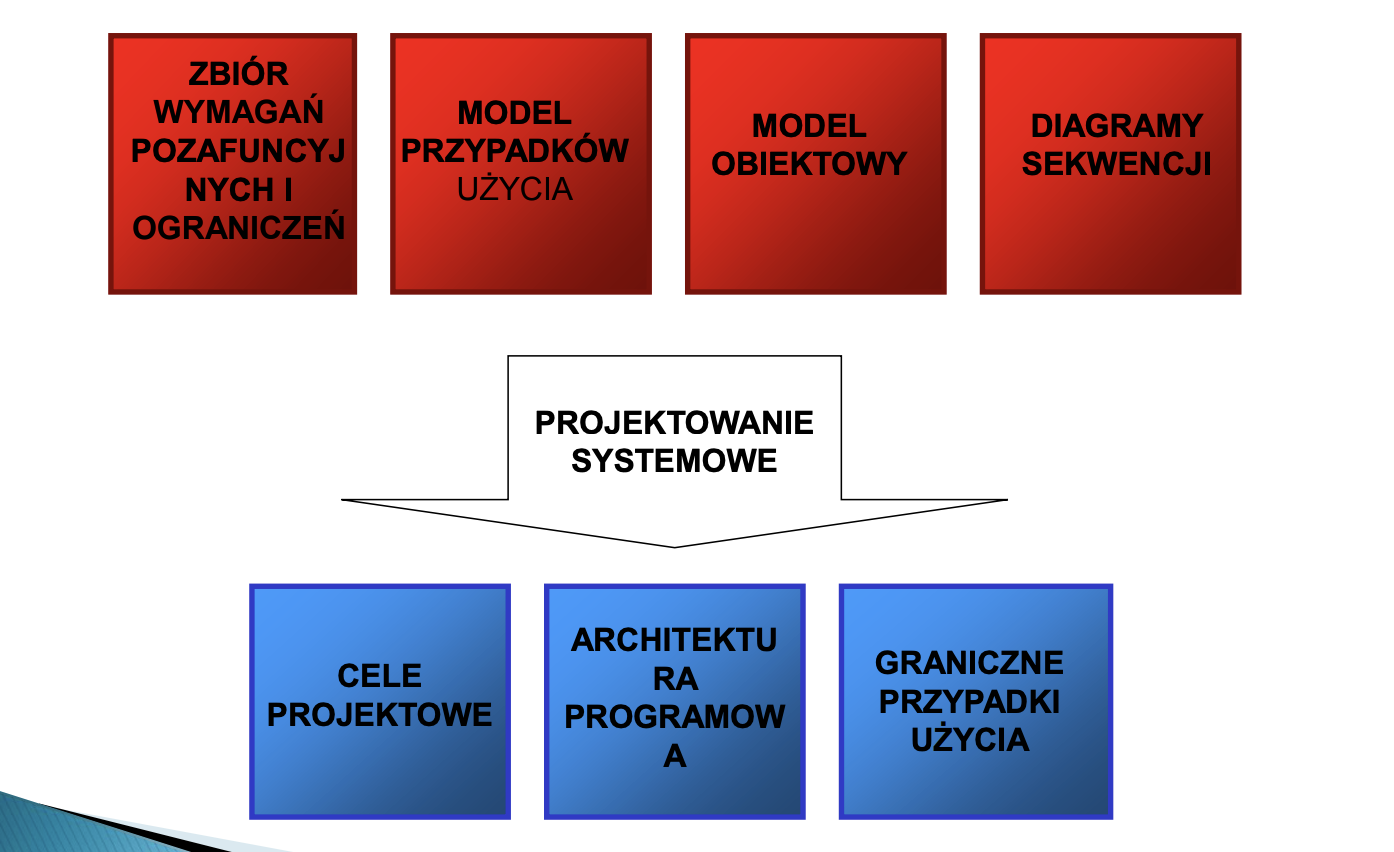
\includegraphics[width=\linewidth]{projekt_systemu.png}
    \end{figure}

    \subsection{Podstawowe pojęcia i koncepcje.}
    \begin{itemize}
        \item \textbf{Podsystem} - wymienna część systemu, posiadającą dobrze zdefiniowane interfejsy i
        hermetyzującą stan oraz zachowanie składających się na nią klas.
        \item Dwa główne typy komponentów: \textbf{logiczny i fizyczny}.
        \item \textbf{Usługa} jest zbiorem powiązanych operacji podporządkowanych realizacji wspólnego
        celu.
        \item \textbf{Sprzężeniem} w zbiorze podsystemów nazywamy stopień ich \textbf{wzajemnego uzależnienia}. (MINIMALIZACJA)
        \item \textbf{Spoistość} podsystemu jest miara \textbf{uzależnienia jego własnych klas}. (MAKSYMALIZACJA)
        \item \textbf{Warstwa} - zgrupowanie podsystemów oferujących powiązane usługi.
        \item Efektem \textbf{dekompozycji hierarchicznej} jest uporządkowany zbiór warstw.
        \item \textbf{Architektury warstwowa}: otwarta i zamknięta (np. ISO/OSI, TCP/IP).
    \end{itemize}


    \subsection{Wzorce architektoniczne - poziom integracji komponentów}

    \subsubsection{MVC: model-widok-kontroler}
    Model zawiera podstawową funkcjonalność. Widoki wyświetlają funkcjonalności. Kontroler obsługuje żądanie użytkownika. Kontroler z widokami tworzą UI aplikacji.

    Zastosowania: Smalltalk, Java/Swing.

    \begin{figure}[H]
        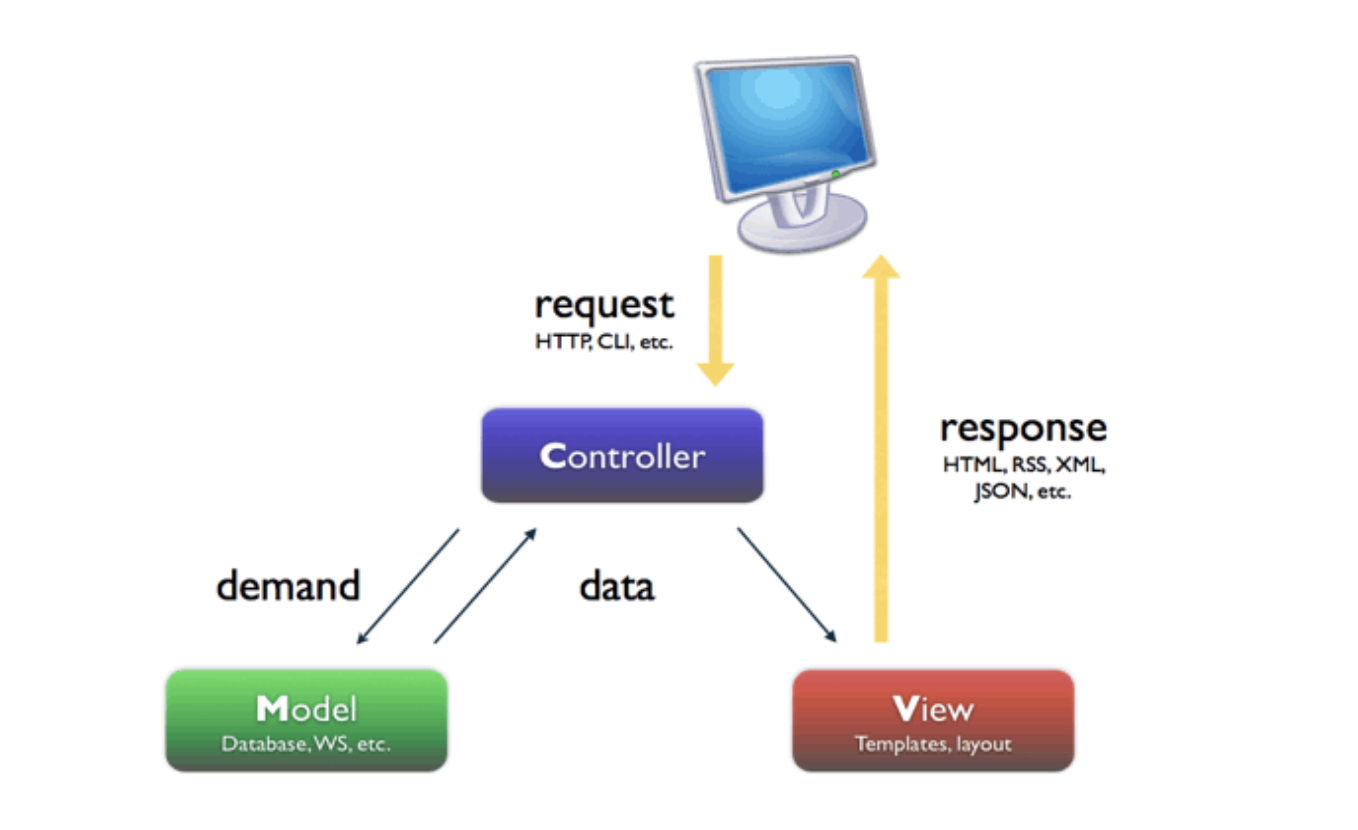
\includegraphics[width=.5\linewidth]{mvc.png}
        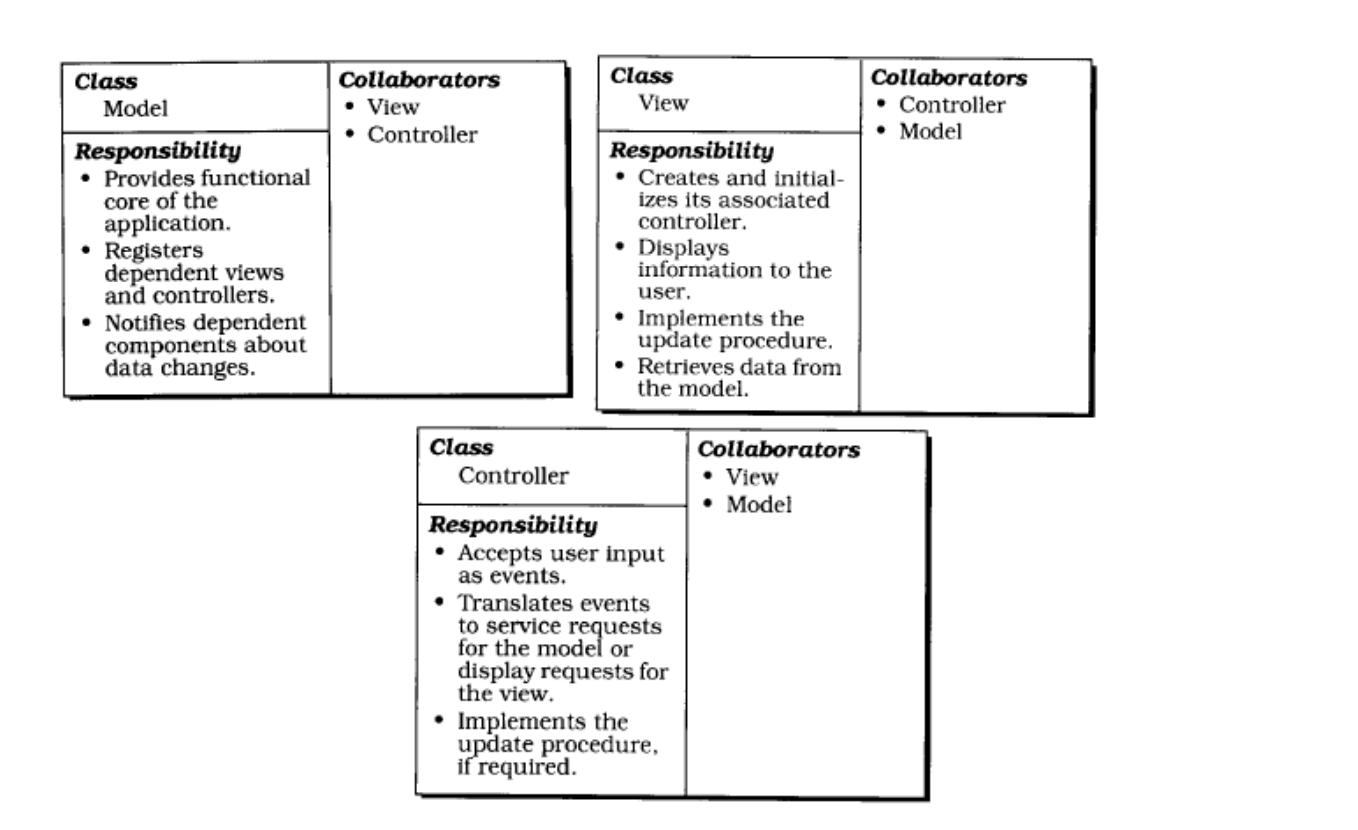
\includegraphics[width=.5\linewidth]{mvc-struktura.png}
    \end{figure}



    \subsubsection{PAC: prezentacja-abstrakcja-kontrola}
    Hierarchie kooperujących agentów, podzielonych na trzy komponenty: prezentacji, abstrakcji, kontroli.

    Zastosowania: Network Traffic Management (gathering traffic data, displaying various user-configurable
    views of the whole network).

    \begin{figure}[h]
        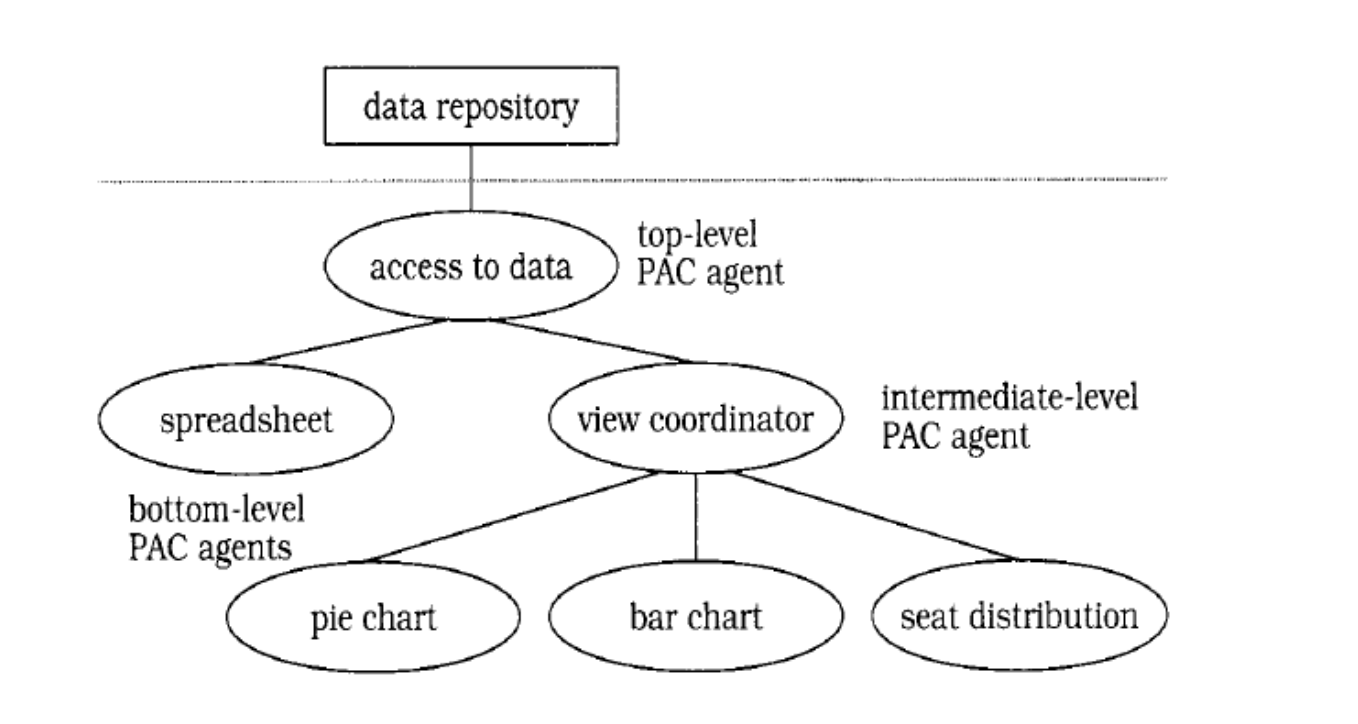
\includegraphics[width=.5\linewidth]{pac.png}
        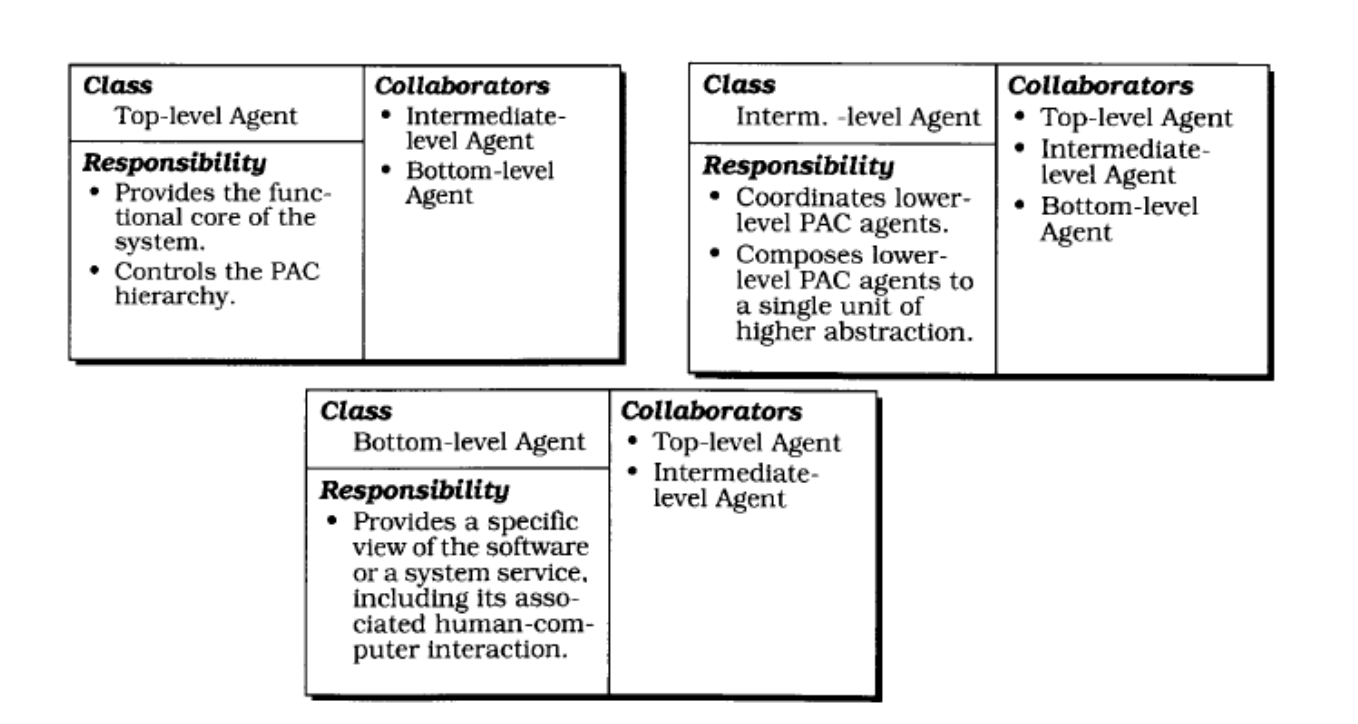
\includegraphics[width=.5\linewidth]{pac-struktura.png}
    \end{figure}



    \subsubsection{Architektura filtry i potoki}

    Pozwala na uporządkowanie systemu, który przetwarza strumienie danych. Każdy krok przetwarzania jest zamknięty w filtrze.
    Dane są przesyłane za pomocą potoków. Każdy z podsystemów realizuje przetwarzanie danych otrzymanych od innych podsystemów.

    Zastosowania: Unix, WEB, Servlet, Numerical Analysis (filters and data extractions).

    \begin{figure}[h]
        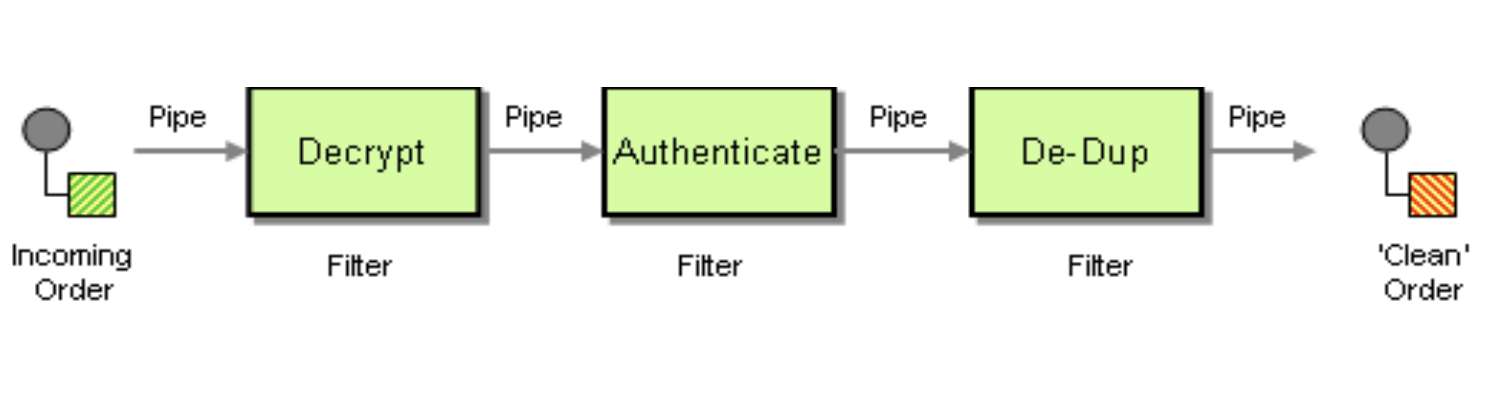
\includegraphics[width=.5\linewidth]{fip.png}
        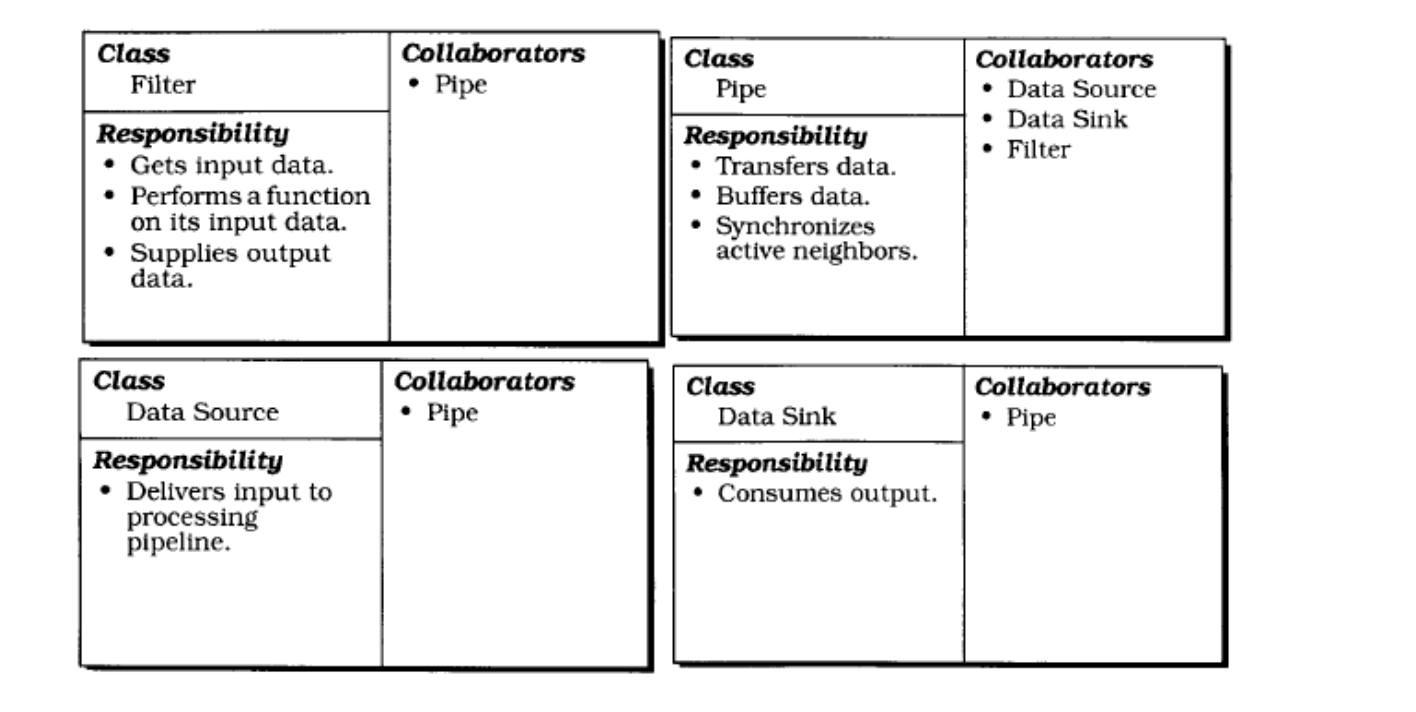
\includegraphics[width=.5\linewidth]{fip_struktura.png}
    \end{figure}




    \subsubsection{Tablica (blackboard)}
    Użyteczna w systemach, gdzie nie są znane deterministyczne rozwiązania danego problemu. W przypadku tablicy kilka wyspecjalizowanych
    systemów łączy swoją wiedzę w taki sposób, żeby stworzyć częściowe lub przybliżone rozwiązanie problemu.

    Zastosowania: working memory, repository data.

    \begin{figure}[h]
        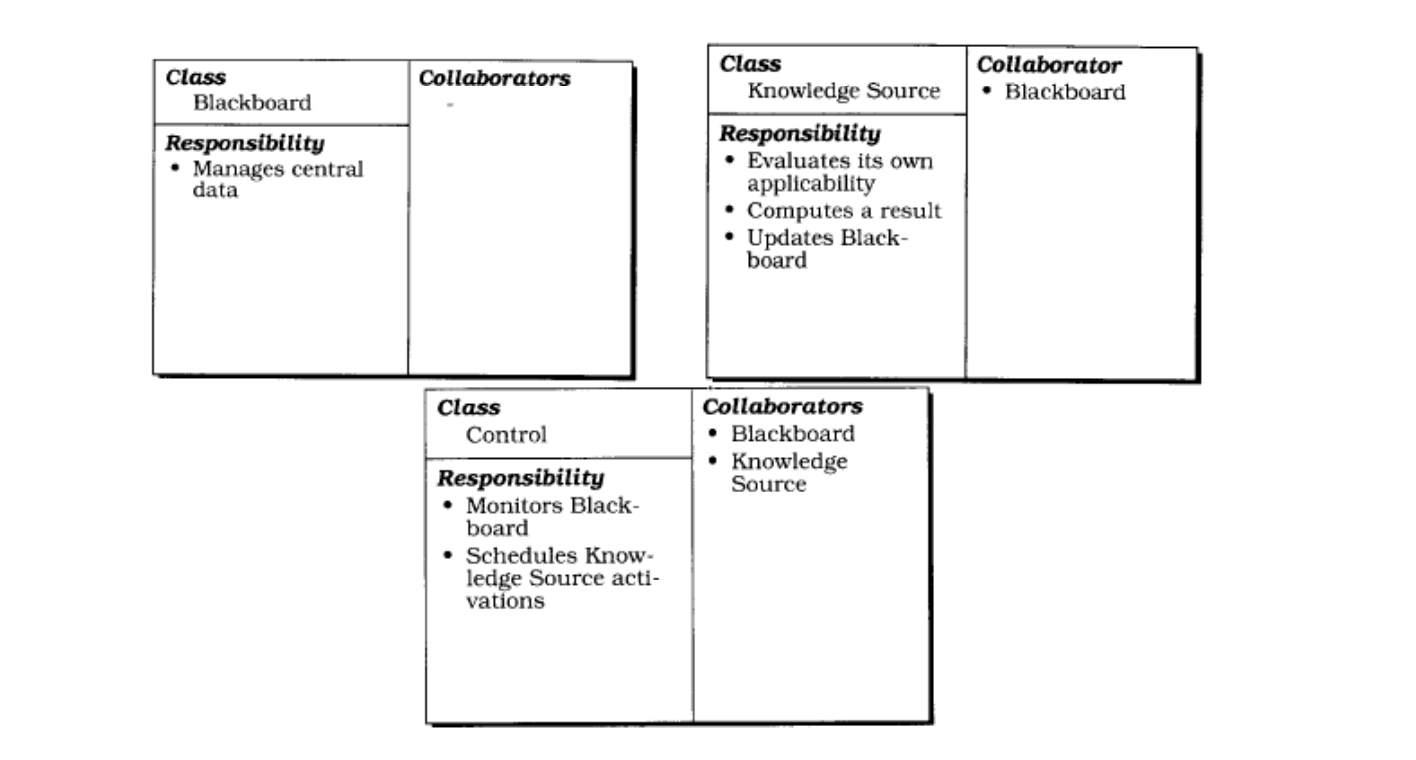
\includegraphics[width=.5\linewidth]{tablica.png}
    \end{figure}



    \subsubsection{Broker}
    Pozwala na uporządkowanie rozproszonych systemów podzielonych na komponenty współpracujące ze sobą za pomocą zdalnego wywoływania
    serwisu. Komponent brokera odpowiedzialny jest za koordynację komunikacji.

    \begin{figure}[h]
        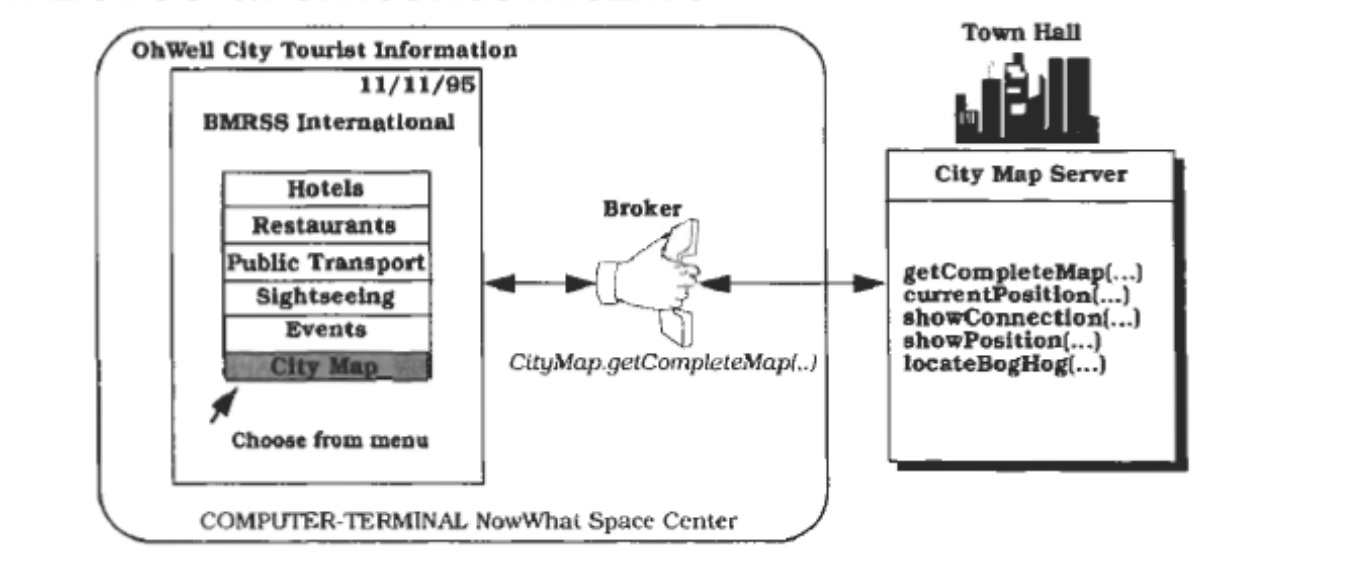
\includegraphics[width=.5\linewidth]{broker.png}
        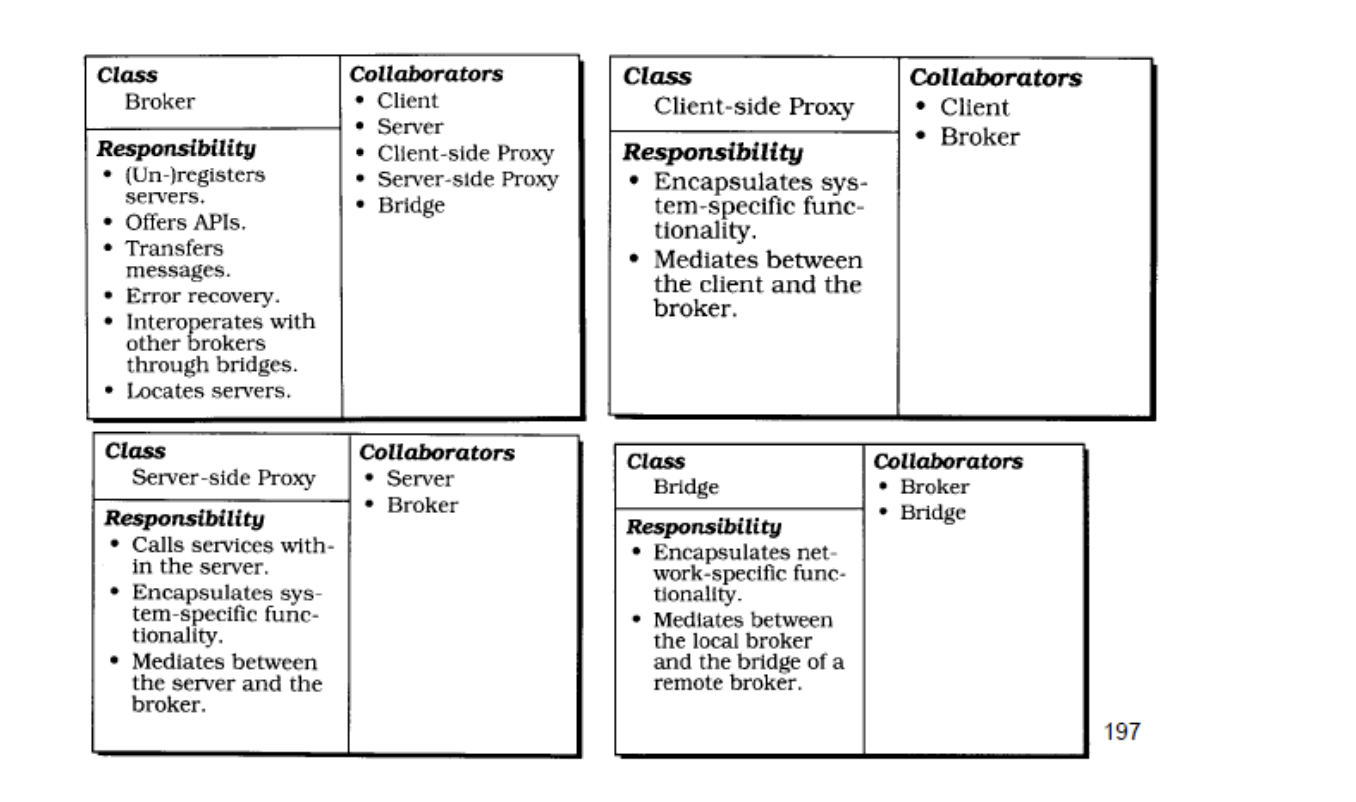
\includegraphics[width=.5\linewidth]{broker_struktura.png}
    \end{figure}

    \subsubsection{Reflection}
    Dostarcza mechanizm pozwalający na dynamiczną zmianę zachowania i struktury systemu.
    \begin{figure}[h]
        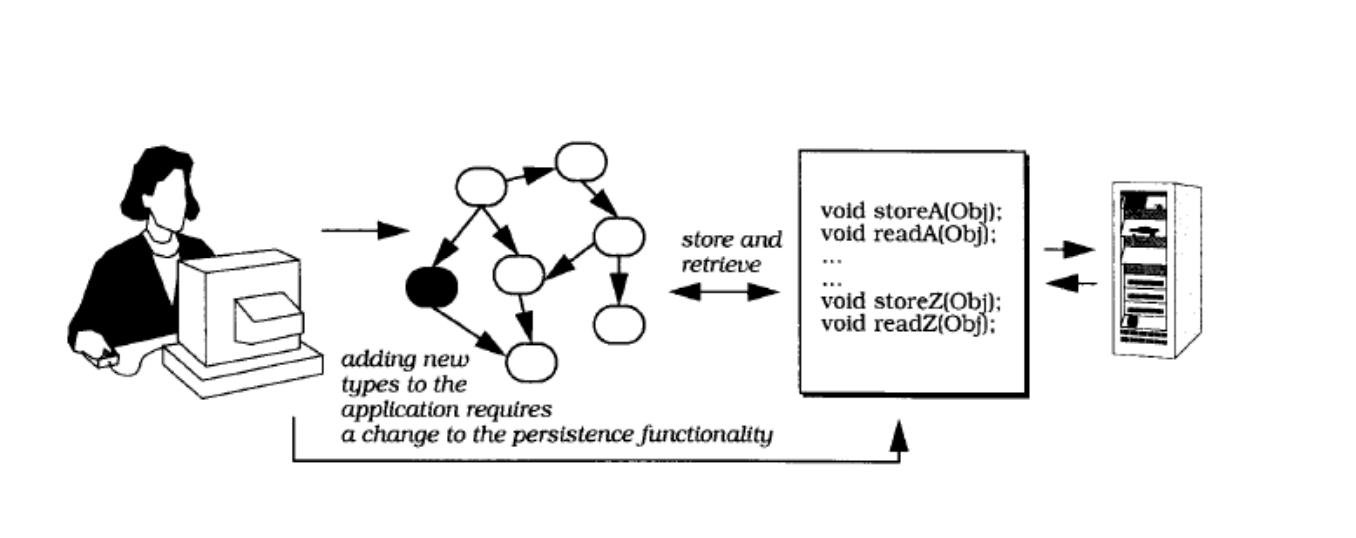
\includegraphics[width=.5\linewidth]{ref.png}
        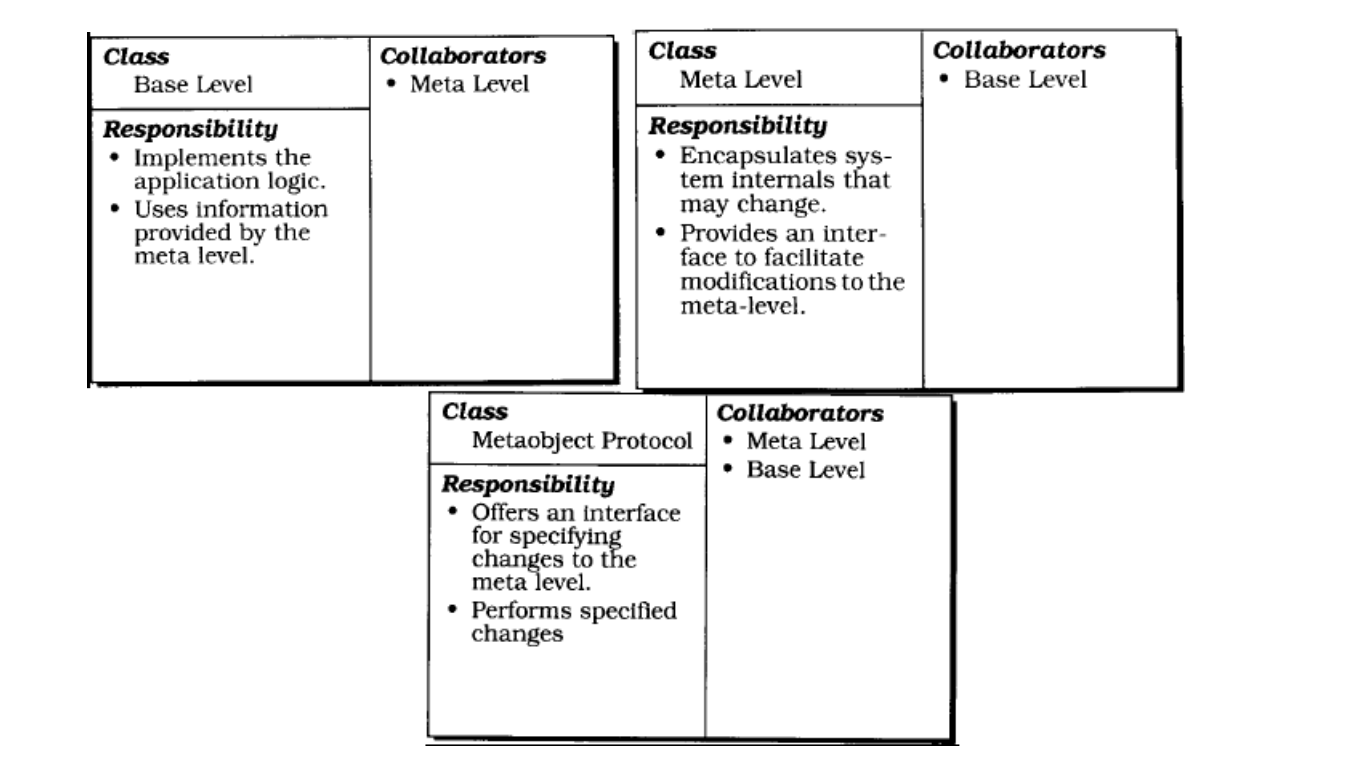
\includegraphics[width=.5\linewidth]{ref_struktura.png}
    \end{figure}

    Zastosowania: WWW.

    \subsubsection{Sieciowe}
    \begin{itemize}
        \item \textbf{Architektura klient-serwer} - podział systemu na dostawce usług (serwer) oraz ich odbiorców (klientów).
        \item \textbf{Architektura peer-to-peer} - każdy z podsystemów może spełniać obie funkcje (klient/serwer).

    \end{itemize}

    \subsubsection{Wzorce architektoniczne - wady}
    \begin{itemize}
        \item Patterns do not lead to direct code reuse.
        \item Individual Patterns are deceptively simple.
        \item Composition of different patterns can be very complex.
        \item Teams may suffer from pattern overload.
        \item Patterns are validated by experience and discussion
        rather than by automated testing.
        \item Integrating patterns into a software development
        process is a human-intensive activity.
    \end{itemize}


\end{document}
